\definecolor{acmBlue}{HTML}{1F77B4}
\definecolor{acmSand}{HTML}{D55E00}
\definecolor{acmGrid}{HTML}{D9DDE2}
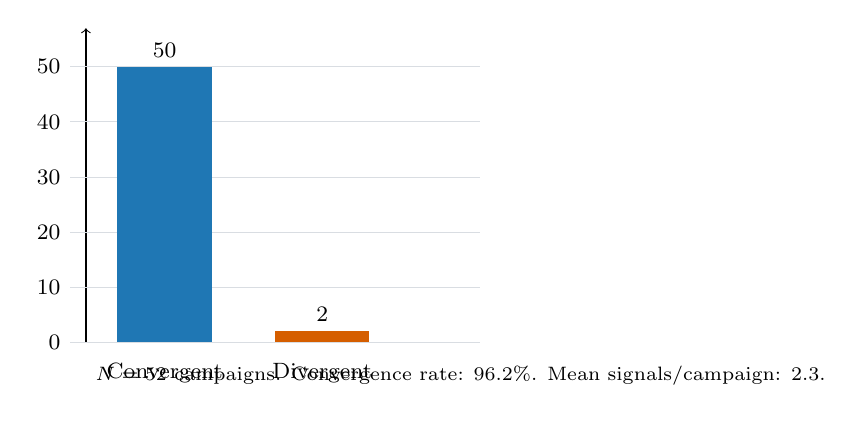
\begin{tikzpicture}[x=2.0cm,y=0.07cm,font=\footnotesize]
  \draw[->] (0,0) -- (0,57);
  \draw[acmGrid] (-0.1,0) -- (2.5,0);
  \node[left] at (-0.1,0) {0};
  \draw[acmGrid] (-0.1,10) -- (2.5,10);
  \node[left] at (-0.1,10) {10};
  \draw[acmGrid] (-0.1,20) -- (2.5,20);
  \node[left] at (-0.1,20) {20};
  \draw[acmGrid] (-0.1,30) -- (2.5,30);
  \node[left] at (-0.1,30) {30};
  \draw[acmGrid] (-0.1,40) -- (2.5,40);
  \node[left] at (-0.1,40) {40};
  \draw[acmGrid] (-0.1,50) -- (2.5,50);
  \node[left] at (-0.1,50) {50};
  \fill[acmBlue] (0.2,0) rectangle (0.8,50);
  \node[above] at (0.5,50) {50};
  \node[below] at (0.5,-2) {Convergent};
  \fill[acmSand] (1.2,0) rectangle (1.8,2);
  \node[above] at (1.5,2) {2};
  \node[below] at (1.5,-2) {Divergent};
  \node[anchor=west,font=\scriptsize] at (0,-6) {$N=52$ campaigns. Convergence rate: 96.2\%. Mean signals/campaign: 2.3.};
\end{tikzpicture}
